\documentclass{article}

\usepackage{geometry}
\usepackage{amsmath}
\usepackage{graphicx, eso-pic}
\usepackage{listings}
\usepackage{hyperref}
\usepackage{multicol}
\usepackage{fancyhdr}
\pagestyle{fancy}
\fancyhf{}
\hypersetup{ colorlinks=true, linkcolor=black, filecolor=magenta, urlcolor=cyan}
\geometry{ a4paper, total={170mm,257mm}, top=40mm, right=20mm, bottom=20mm, left=20mm}
\setlength{\parindent}{0pt}
\setlength{\parskip}{0.5em}
\renewcommand{\headrulewidth}{0pt}
\AddToShipoutPictureBG{%
  \AtPageUpperLeft{%
    \raisebox{-\height}{
\includegraphics[width=\paperwidth, height=30mm]{../headerarkav.png}}
  }
}
\rfoot{\thepage}
\lfoot{Competitive Programming - Arkavidia 8.0}
\lstset{
    basicstyle=\ttfamily\small,
    columns=fixed,
    extendedchars=true,
    breaklines=true,
    tabsize=2,
    prebreak=\raisebox{0ex}[0ex][0ex]{\ensuremath{\hookleftarrow}},
    frame=none,
    showtabs=false,
    showspaces=false,
    showstringspaces=false,
    prebreak={},
    keywordstyle=\color[rgb]{0.627,0.126,0.941},
    commentstyle=\color[rgb]{0.133,0.545,0.133},
    stringstyle=\color[rgb]{01,0,0},
    captionpos=t,
    escapeinside={(\%}{\%)}
}

\begin{document}

\begin{center}
    \section*{G. Gedung Susun} % ganti judul soal

    \begin{tabular}{ | c c | }
        \hline
        Batas Waktu  & 2s \\    % jangan lupa ganti time limit
        Batas Memori & 256MB \\  % jangan lupa ganti memory limit
        \hline
    \end{tabular}
\end{center}

\subsection*{Deskripsi}
Arka tinggal di sebuah kompleks gedung yang berderet di sepanjang jalan. Kompleks gedung ini memiliki tepat $N$ buah gedung dan setiap gedung memiliki $M$ buah lantai. Untuk meningkatkan keeratan hubungan antar gedung, desain infrastruktur kompleks gedung ini cukup unik. Setiap gedung dinomori dari $1$ sampai $N$ dari kiri ke kanan dan setiap lantai pada sebuah gedung dinomori dari $1$ ke $M$ dari bawah ke atas. Setiap gedung yang bersebelahan dihubungkan dengan sebuah jembatan di setiap lantainya. 

Untuk memaksimalkan kenyamanan gedung, \textit{ground floor} untuk gedung ke-$i$ dipilih pada nomor lantai $GF_{i}$. Adapun untuk mengakses gedung ke-$i$, pengunjung perlu membayarkan biaya dasar sebesar $B_{i}$. Selain itu, untuk mengakses lantai ke-$j$ pada gedung ke-${i}$, diperlukan biaya tambahan sebesar $|j - GF_{i}|$ saat pertama kali memasuki gedung. Setiap gedung juga difasilitasi dengan sebuah elevator yang dapat diakses pada lantai manapun di gedung tersebut. Namun, untuk menggunakan elevator, pengunjung perlu membayar sejumlah lantai yang dilalui oleh elevator, dengan kata lain penggunaan elevator dari lantai ke-$k$ menuju lantai ke-$j$ diperlukan biaya sebesar $|k-j|$.

Arka ingin berangkat dari gedung tempat ia tinggal di gedung ke-$1$ menuju gedung kantor tempatnya bekerja di gedung ke-$N$. Namun, saat ini elevator setiap gedung sedang dalam masa perawatan, sehingga setiap gedung membatasi setiap orang untuk menggunakan elevator tidak lebih dari satu kali. Selain itu, pada gedung ke-$i$, penggunaan elevator hanya bisa naik atau turun sebanyak $D_{i}$ lantai, sehingga akses elevator pada lantai ke-$j$ dapat menuju lantai ke-$k$ hanya jika $|k-j|\leq D_{i}$.

Karena sedang tanggal tua, Arka ingin meminimumkan biaya yang ia keluarkan untuk mencapai kantornya. Arka meminta bantuan Anda untuk mencari biaya minimum yang perlu Arka siapkan jika Arka dapat memulai perjalanannya dari lantai mana saja di gedung tempat ia tinggal. Selain itu, kantor tempat Arka bekerja sudah membiayai akses elevator di gedung kantor, sehingga Arka hanya perlu mengetahui biaya total hingga sampai di gedung kantor pada lantai manapun.

\subsection*{Format Masukan}
Baris pertama terdiri dari dua buah bilangan bulat positif $N$ ($2 \leq N \leq 10^5$) dan $M$ ($2 \leq M \leq 100$) yang menyatakan banyaknya gedung dan banyaknya lantai.

Baris kedua berupa $N$ buah bilangan $GF_1, GF_2, \dots, GF_N$ ($1 \leq GF_{i} \leq M$) yang menyatakan \textit{ground floor} dari gedung ke-$i$.

Baris ketiga berupa $N$ buah bilangan $B_1, B_2, \dots, B_N$ ($0 \leq B_{i} \leq 10^9$) yang menyatakan biaya dasar akses gedung ke-$i$.

Baris keempat berupa $N$ buah bilangan $D_1, D_2, \dots, D_N$ ($1 \leq D_{i} \leq M-1$) yang menyatakan banyaknya lantai maksimal yang bisa dilalui elevator pada gedung ke-$i$.

\subsection*{Format Keluaran}
Sebuah baris yang menyatakan biaya minimum untuk mencapai gedung ke-$N$ dari gedung ke-$1$.

\begin{multicols}{2}
\subsection*{Contoh Masukan 1}
\begin{lstlisting}
2 2
1 2
10 8
1 1
\end{lstlisting}
\columnbreak
\subsection*{Contoh Keluaran 1}
\begin{lstlisting}
19
\end{lstlisting}
\vfill
\null
\end{multicols}

\begin{multicols}{2}
\subsection*{Contoh Masukan 2}
\begin{lstlisting}
4 5
4 2 1 4
11 12 7 6
1 4 2 1
\end{lstlisting}
\columnbreak
\subsection*{Contoh Keluaran 2}
\begin{lstlisting}
41
\end{lstlisting}
\vfill
\null
\end{multicols}

\subsection*{Penjelasan}
Misalnya $(p, q)$ menyatakan bahwa Arka melewati gedung ke-$p$ di lantai ke-$q$. 

Pada testcase pertama, salah satu cara Arka mencapai gedung kantornya dengan biaya minimal adalah melalui $(1, 1) \xrightarrow{} (1, 2) \xrightarrow{} (2, 2) $. Biaya akses gedung total adalah $B_{1}+B_{2} = 10+8=18$. Biaya elevator menuju lantai $2$ di gedung ke-$1$ adalah $|2-1|=1$. Adapun biaya lantai setiap gedung adalah $|1-1|+|2-2|=0$. Dengan demikian, total biaya yang diperlukan adalah $1 + 18 + 0 = 19$. Dapat dibuktikan bahwa tidak ada cara bagi Arka untuk mendapatkan biaya lebih murah dari $19$.\newline

Pada testcase kedua, perhatikan ilustrasi berikut. Lantai berwarna merah adalah \textit{ground floor} dari gedung tersebut. 
\begin{center}
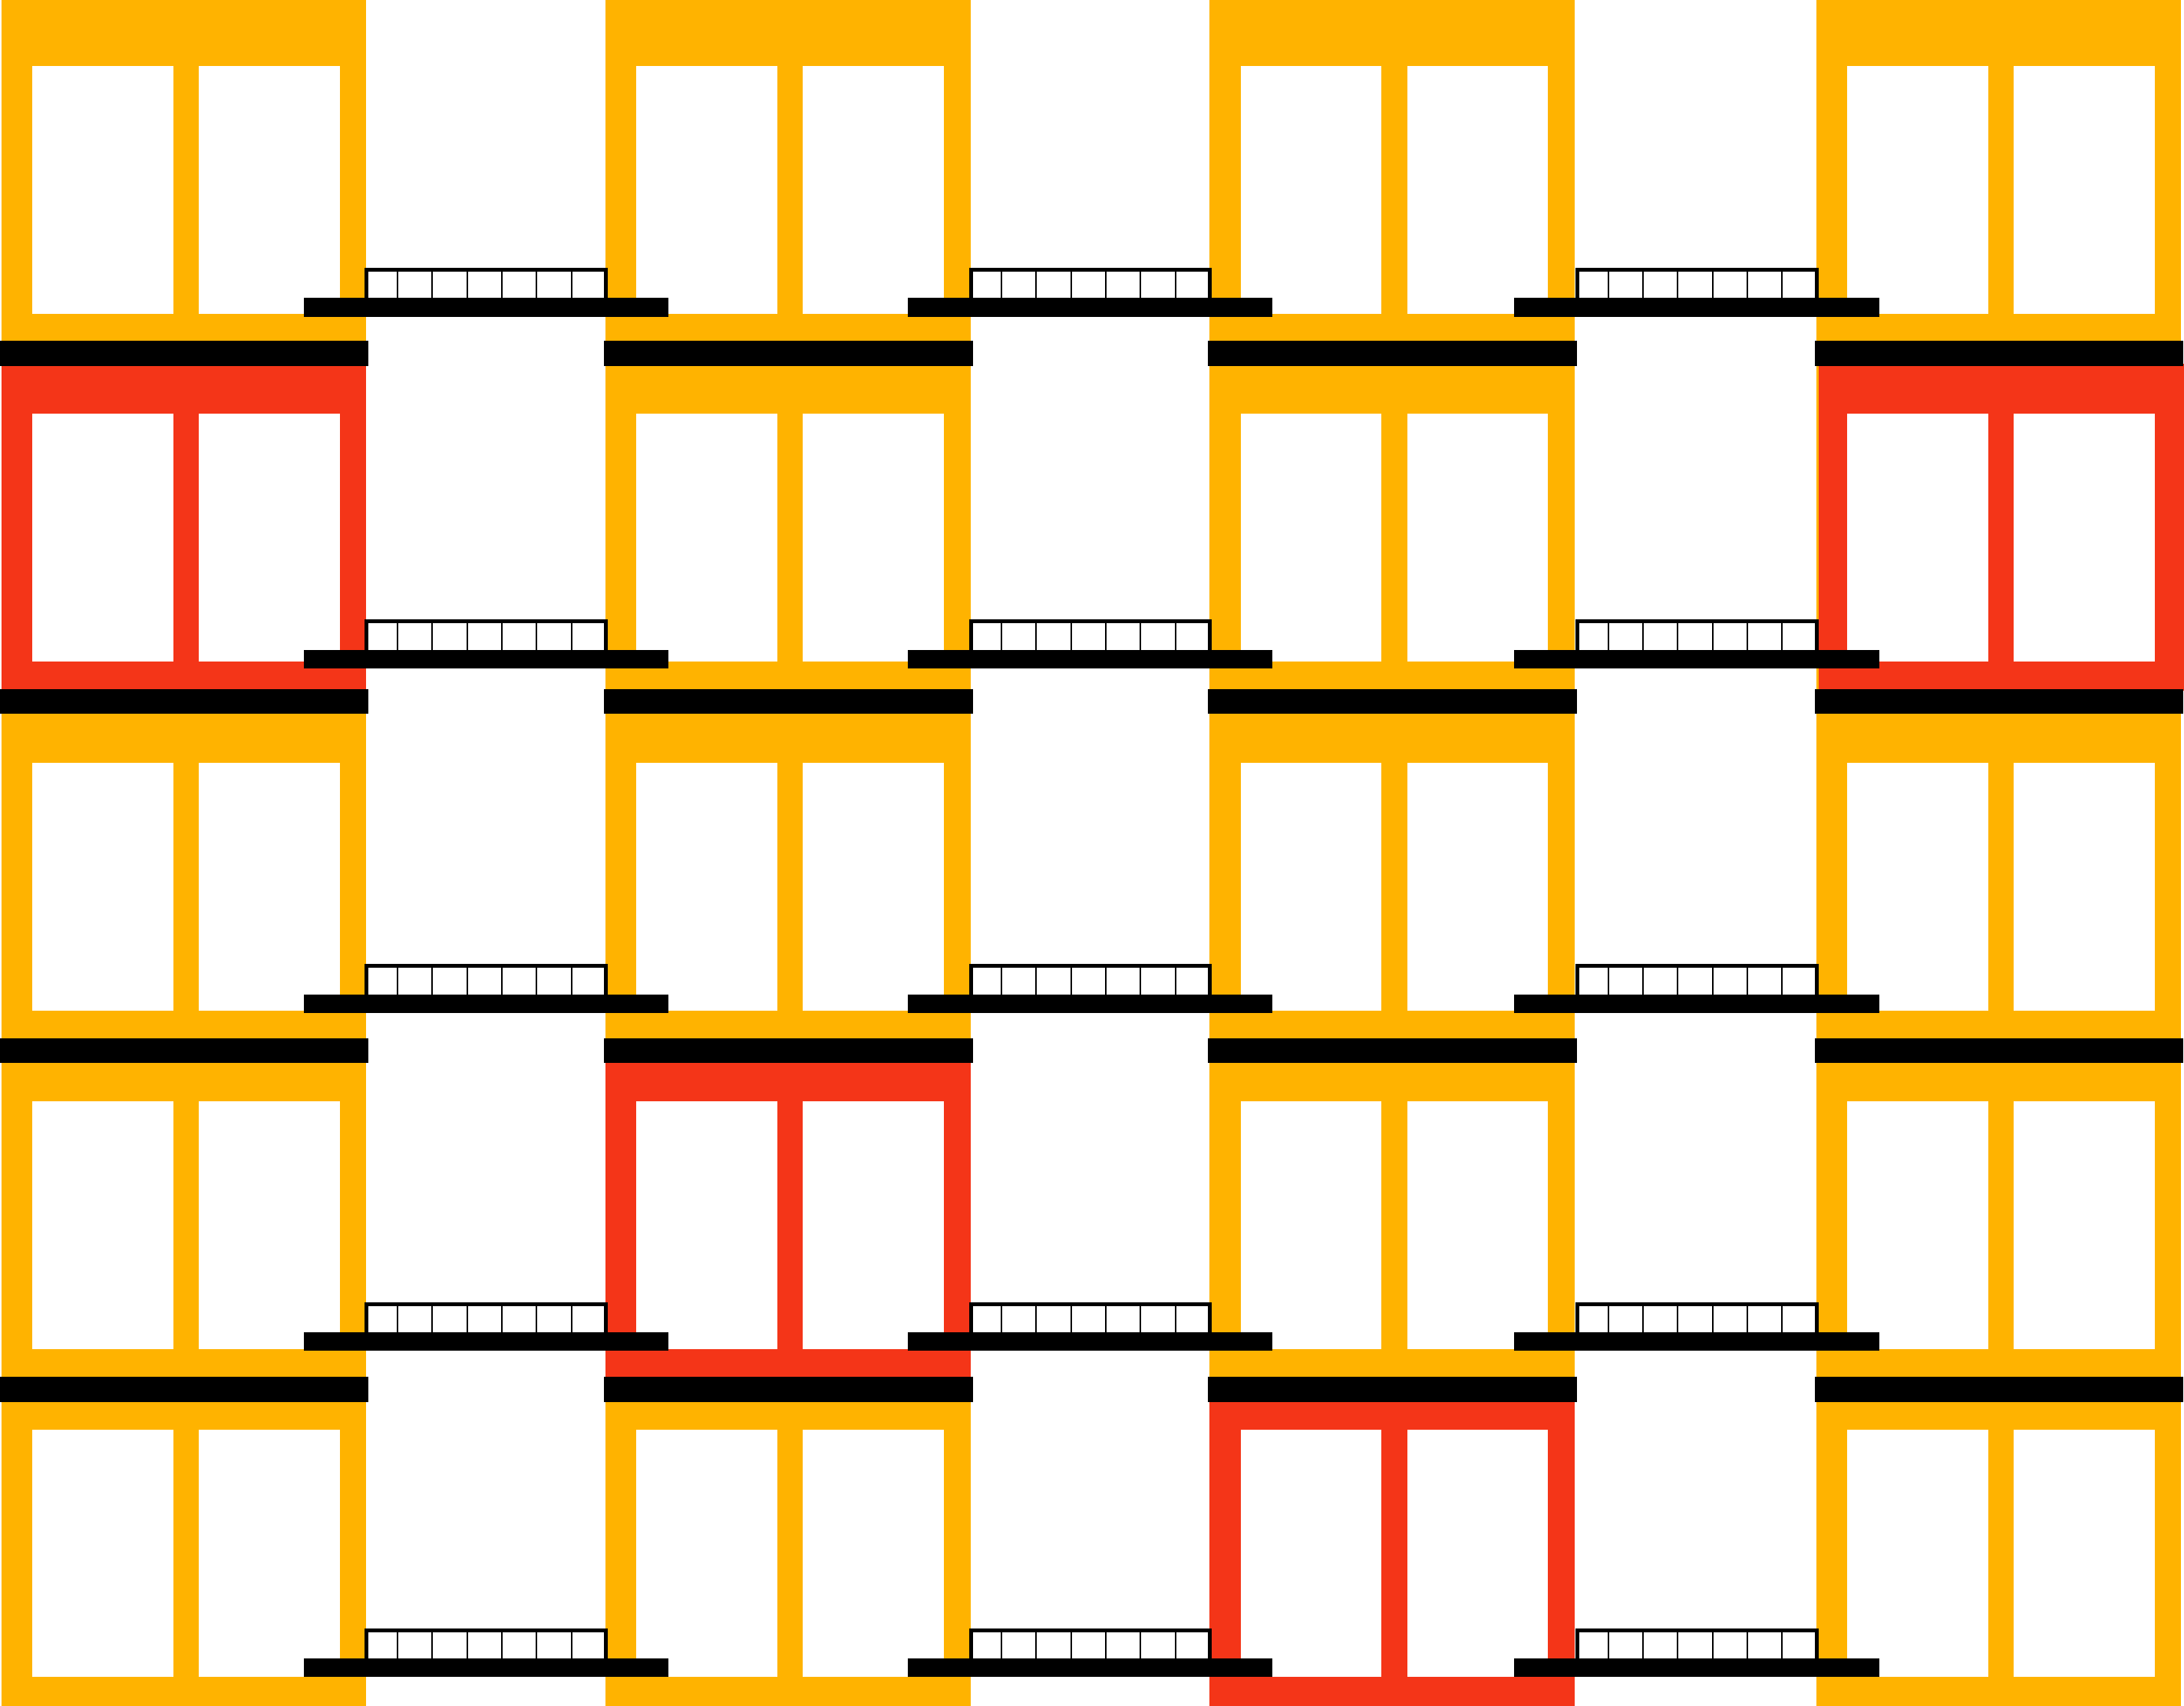
\includegraphics[height=200px]{ilustrasi-1.png}
\end{center}
Salah satu cara Arka dapat mencapai gedung ke-$N$ dengan biaya minimal adalah $(1, 3) \xrightarrow{} (1, 2) \xrightarrow{} (2, 2) \xrightarrow{} (3, 2) \xrightarrow{} (3, 3) \xrightarrow{} (4, 3)$. Biaya akses total gedung adalah $B_{1}+B_{2}+B_{3}+B_{4} = 36$. Biaya elevator dari gedung ke-$1$ dari lantai $3$ menuju lantai $2$ dan gedung ke-$3$ dari lantai $2$ menuju lantai $3$ adalah $|3-2| + |2-3| = 2$. Biaya lantai gedung adalah $|3-4| + |2-2| + |2-1| + |3-4| = 3$. Sehingga total biayanya adalah $41$. Dapat dibuktikan bahwa tidak ada cara lain bagi Arka untuk mendapatkan biaya total lebih kecil dari $41$.

\end{document}